\documentclass[border=10pt]{standalone}
\usepackage[svgnames]{xcolor}
\usepackage{amsmath}
\usepackage{pgfplots}
\pgfplotsset{compat=newest}
\usepackage[sfdefault]{FiraSans}
\usepackage{FiraMono}
\renewcommand*\familydefault{\sfdefault}
\begin{document}
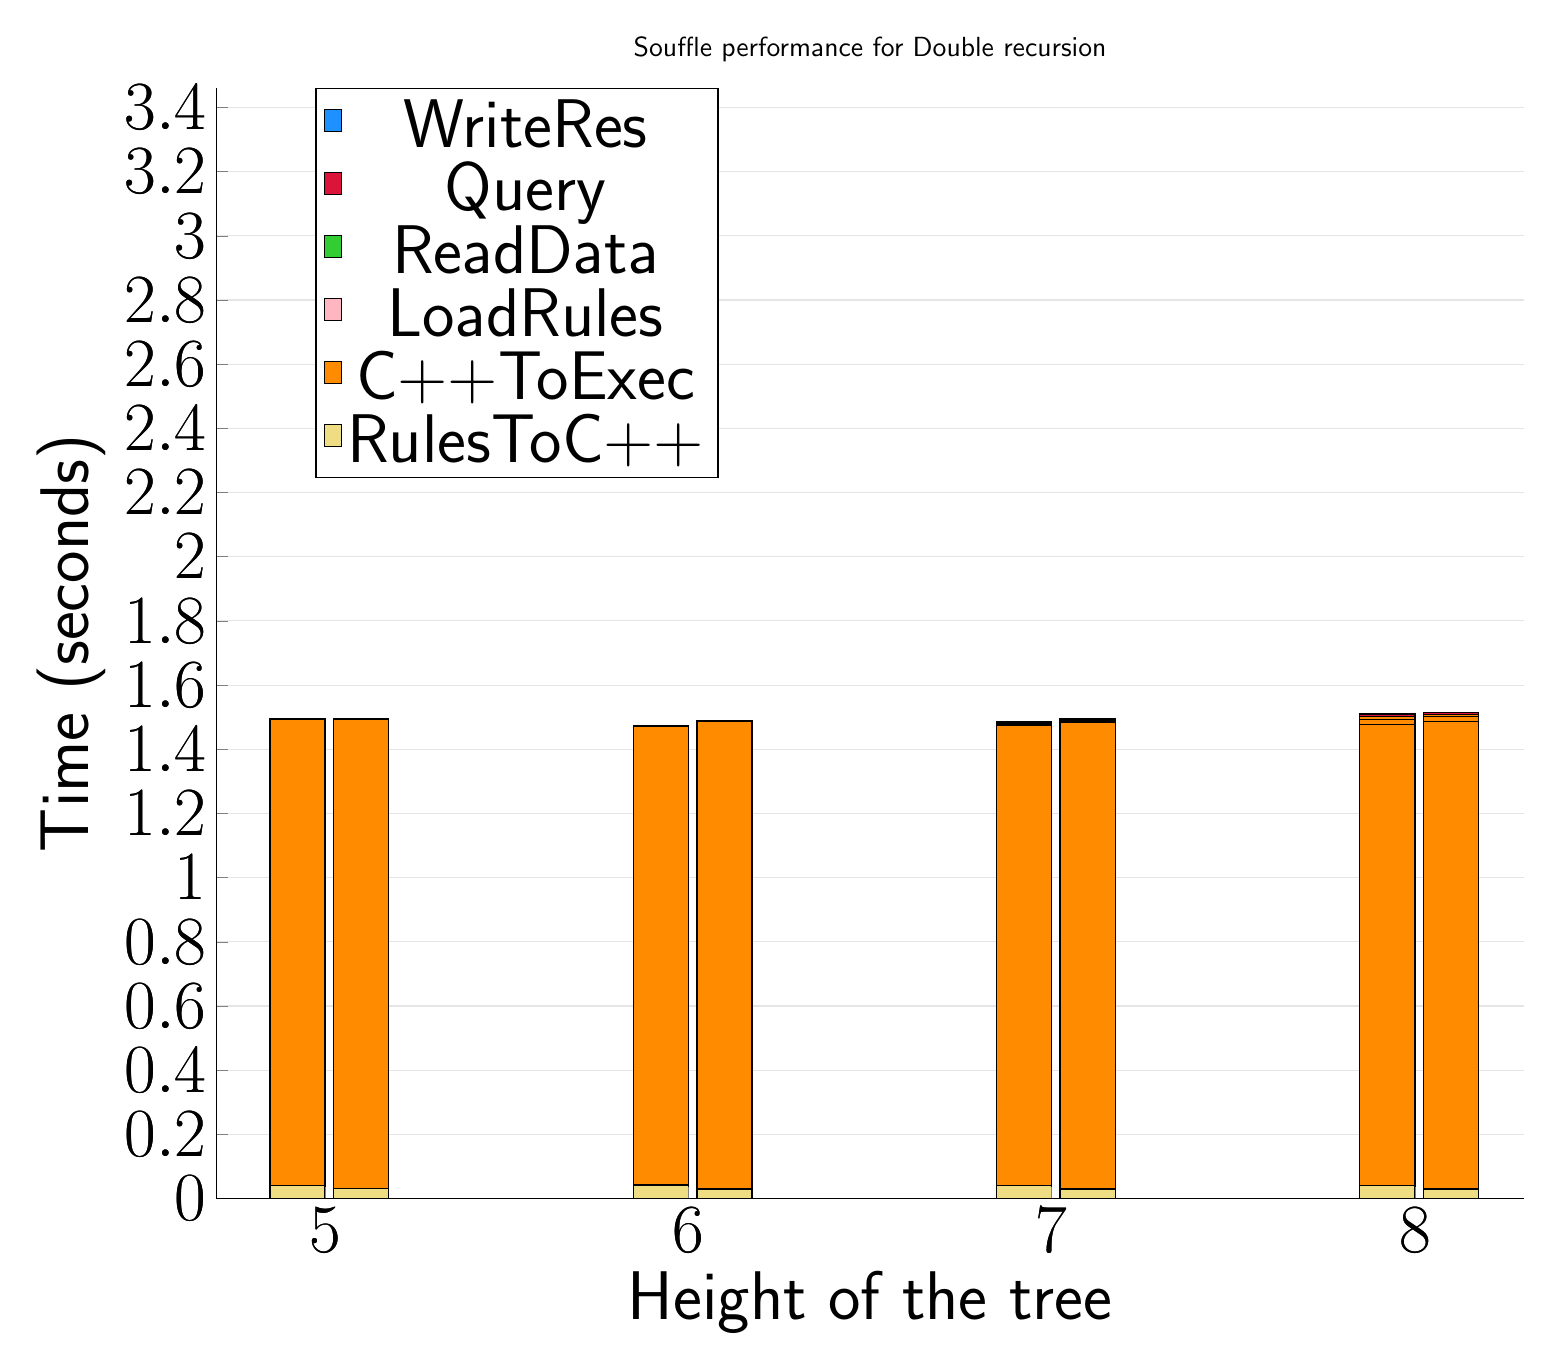
\begin{tikzpicture}
\begin{axis}[
   ybar stacked,
   title={Souffle performance for Double recursion},
   bar shift=-10pt,
   width=1.5\textwidth,
   bar width=0.7cm,
   ymajorgrids, tick align=inside,
   major grid style={draw=gray!20},
   xtick=data,
   ymin=0, ymax=3.4609999895095824,
   axis x line*=bottom,
   axis y line*=left,
   enlarge x limits=0.1,
   legend style={
       at={(0.23, 1)},
       anchor=north,
       legend columns=1,
       font=\Huge,
   },
   ylabel={Time (seconds)},
   xlabel={Height of the tree},
   label style={font=\Huge},
   tick label style={font=\Huge},
]
\addlegendimage{fill=DodgerBlue, draw=black, line width=0.2pt}
\addlegendentry{WriteRes}
\addlegendimage{fill=Crimson, draw=black, line width=0.2pt}
\addlegendentry{Query}
\addlegendimage{fill=LimeGreen, draw=black, line width=0.2pt}
\addlegendentry{ReadData}
\addlegendimage{fill=LightPink, draw=black, line width=0.2pt}
\addlegendentry{LoadRules}
\addlegendimage{fill=DarkOrange, draw=black, line width=0.2pt}
\addlegendentry{C++ToExec}
\addlegendimage{fill=LightGoldenrod, draw=black, line width=0.2pt}
\addlegendentry{RulesToC++}
\addplot +[fill=LightGoldenrod, draw=black, line width=0.5pt] coordinates {
    (5, 0.039999985694885255)
    (6, 0.041999983787536624)
    (7, 0.04100000858306885)
    (7, 0.04100000858306885)
    (7, 0.039999985694885255)
    (8, 0.039999985694885255)
    (8, 0.04100000858306885)
    (8, 0.04100000858306885)
};
\addplot +[fill=DarkOrange, draw=black, line width=0.5pt] coordinates {
    (5, 1.453000020980835)
    (6, 1.4300000429153443)
    (7, 1.434000015258789)
    (7, 1.4410000085830688)
    (7, 1.4380000114440918)
    (8, 1.452999997138977)
    (8, 1.4609999895095824)
    (8, 1.4360000371932984)
};
\addplot +[fill=LightPink, draw=black, line width=0.5pt] coordinates {
    (5, 0.00012735840000000002)
    (6, 0.00011126250000000001)
    (7, 0.00011146679999999998)
    (7, 0.0001089793)
    (7, 0.0001207582)
    (8, 0.0001111251)
    (8, 0.0001257958)
    (8, 0.00012474159999999998)
};
\addplot +[fill=LimeGreen, draw=black, line width=0.5pt] coordinates {
    (5, 0.0003257125)
    (6, 0.0003901249)
    (7, 0.0005279208)
    (7, 0.0005145708000000001)
    (7, 0.0005086709)
    (8, 0.0007638251)
    (8, 0.0008131917)
    (8, 0.0008116663999999999)
};
\addplot +[fill=Crimson, draw=black, line width=0.5pt] coordinates {
    (5, 0.00027294159999999995)
    (6, 0.0008180125999999999)
    (7, 0.00216813)
    (7, 0.002084159)
    (7, 0.002074624)
    (8, 0.0054718119999999995)
    (8, 0.005653554)
    (8, 0.005618446)
};
\addplot +[fill=DodgerBlue, draw=black, line width=0.5pt] coordinates {
    (5, 0.00038823739999999996)
    (6, 0.0004931908)
    (7, 0.0005637121999999999)
    (7, 0.0007269548000000001)
    (7, 0.0005900377)
    (8, 0.0009430628999999999)
    (8, 0.0009521290999999999)
    (8, 0.0009799961)
};
\end{axis}
\begin{axis}[
   ybar stacked,
   bar shift=13pt,
   width=1.5\textwidth,
   bar width=0.7cm,
   ymajorgrids, tick align=inside,
   major grid style={draw=none},
   xtick=data,
   ymin=0, ymax=3.4609999895095824,
   axis x line*=none,
   axis y line*=none,
   enlarge x limits=0.1,
   label style={font=\Huge},
   tick label style={font=\Huge},
]
\addplot +[fill=LightGoldenrod, draw=black, line width=0.5pt] coordinates {
    (5, 0.031000000000000007)
    (6, 0.030000000000000006)
    (7, 0.030000000000000006)
    (7, 0.030000000000000006)
    (7, 0.030000000000000006)
    (8, 0.030999999999999993)
    (8, 0.031000000000000007)
    (8, 0.030000000000000006)
};
\addplot +[fill=DarkOrange, draw=black, line width=0.5pt] coordinates {
    (5, 1.4629999999999999)
    (6, 1.457)
    (7, 1.4580000000000002)
    (7, 1.4609999999999999)
    (7, 1.454)
    (8, 1.471)
    (8, 1.4769999999999999)
    (8, 1.4569999999999999)
};
\addplot +[fill=LightPink, draw=black, line width=0.5pt] coordinates {
    (5, 0.0001265)
    (6, 0.0001102)
    (7, 0.00011059999999999998)
    (7, 0.0001081)
    (7, 0.00011980000000000001)
    (8, 0.0001105)
    (8, 0.00012460000000000002)
    (8, 0.0001239)
};
\addplot +[fill=LimeGreen, draw=black, line width=0.5pt] coordinates {
    (5, 0.0003248)
    (6, 0.0003892)
    (7, 0.0005269000000000001)
    (7, 0.0005139)
    (7, 0.0005077)
    (8, 0.0007628)
    (8, 0.0008121000000000002)
    (8, 0.00081)
};
\addplot +[fill=Crimson, draw=black, line width=0.5pt] coordinates {
    (5, 0.0002724)
    (6, 0.0008173000000000002)
    (7, 0.0021675999999999996)
    (7, 0.0020836)
    (7, 0.0020743000000000003)
    (8, 0.0054711000000000004)
    (8, 0.005651700000000001)
    (8, 0.005616800000000001)
};
\addplot +[fill=DodgerBlue, draw=black, line width=0.5pt] coordinates {
    (5, 0.0002803)
    (6, 0.00034350000000000006)
    (7, 0.000501)
    (7, 0.0005005)
    (7, 0.0005020000000000001)
    (8, 0.0008337)
    (8, 0.0009297999999999999)
    (8, 0.0008827000000000002)
};
\end{axis}
\end{tikzpicture}

\end{document}
